\documentclass{beamer}
\usepackage[utf8]{inputenc}
\usetheme{Madrid}
\usecolortheme{default}
\usepackage{amsmath,amssymb,amsfonts,amsthm}
\usepackage{txfonts}
\usepackage{tkz-euclide}
\usepackage{listings}
\usepackage{adjustbox}
\usepackage{array}
\usepackage{tabularx}
\usepackage{gvv}
\usepackage{lmodern}
\usepackage{circuitikz}
\usepackage{tikz}
\usepackage{graphicx}
\setbeamertemplate{page number in head/foot}[totalframenumber]
\usepackage{tcolorbox}
\tcbuselibrary{minted,breakable,xparse,skins}
\definecolor{bg}{gray}{0.95}
\DeclareTCBListing{mintedbox}{O{}m!O{}}{%
  breakable=true,
  listing engine=minted,
  listing only,
  minted language=#2,
  minted style=default,
  minted options={%
    linenos,
    gobble=0,
    breaklines=true,
    breakafter=,,
    fontsize=\small,
    numbersep=8pt,
    #1},
  boxsep=0pt,
  left skip=0pt,
  right skip=0pt,
  left=25pt,
  right=0pt,
  top=3pt,
  bottom=3pt,
  arc=5pt,
  leftrule=0pt,
  rightrule=0pt,
  bottomrule=2pt,
  toprule=2pt,
  colback=bg,
  colframe=orange!70,
  enhanced,
  overlay={%
    \begin{tcbclipinterior}
    \fill[orange!20!white] (frame.south west) rectangle ([xshift=20pt]frame.north west);
    \end{tcbclipinterior}},
  #3,
}
\lstset{
    language=C,
    basicstyle=\ttfamily\small,
    keywordstyle=\color{blue},
    stringstyle=\color{orange},
    commentstyle=\color{green!60!black},
    numbers=left,
    numberstyle=\tiny\color{gray},
    breaklines=true,
    showstringspaces=false,
}
\begin{document}

\title 
{4.3.50}
\date{september 14,2025}


\author 
{Namaswi-EE25BTECH11060}
\frame{\titlepage}
\begin{frame}{Question}
Find the equation of the lines which makes intercepts -3 and 2 on the x and y axes respectively
\end{frame}
\begin{frame}{solution}
Given that line passes through points $\brak{-3,0}$ and $\brak{0,2}$ \\
Let
\[
\begin{array}{|c|c|}
\hline
\text{Vector} & coordinate \\ \hline
\vec{A} & (-3, 0) \\ \hline
\vec{B} & (0, 2) \\ \hline
\vec{n} & (a, b) \\ \hline
\end{array}
\]
As equation of line is given by 
\begin{align}
    \vec{n}^\top \vec{x}=1
\end{align}
\end{frame}
\begin{frame}{Solution}
   So, for $\vec{A}$
 \begin{align}
 \begin{pmatrix}
     a \\ b 
 \end{pmatrix}^\top\begin{pmatrix}
     -3  \\ 0
 \end{pmatrix}=1
  \end{align}
  for $\vec{B}$
 \begin{align}
 \begin{pmatrix}
     a \\ b 
 \end{pmatrix}^\top\begin{pmatrix}
     0  \\  2
 \end{pmatrix}=1\\ 
\end{align}
\end{frame}
\begin{frame}{Solution}
    From 2 and 3\\
    \begin{align}
    \begin{pmatrix}
     -3 & 0 \\
     0 & 2 
 \end{pmatrix}\begin{pmatrix}
     a \\ b 
 \end{pmatrix}=\begin{pmatrix}
     1 \\ 1
 \end{pmatrix}
    \end{align}
In augmented matrix form\\
\begin{align}
\begin{bmatrix}
-3 & 0 & \big| & 1 \\
0 & 2 & \big| & 1
\end{bmatrix}
\end{align}
Divide Row 1 by -3
\begin{align}
\begin{bmatrix}
-1 & 0 & \big| & \frac{1}{3}\\
0 &  2  & \big| & 1
\end{bmatrix}
\end{align}
\end{frame}
\begin{frame}{Solution}
  Divide Row 2 by 2
\begin{align}
\begin{bmatrix}
  -1 & 0 & \big| & \frac{-1}{3}\\
  0  &  1 & \big| & \frac{1}{2}
\end{bmatrix}\\
a=\frac{-1}{3}\; and\; b=\frac{1}{2}\\
\end{align}
So from 1 Equation of line is 
\begin{pmatrix}
    \frac{-1}{3}\\
    \frac{1}{2}
\end{pmatrix}\vec{x}=1
\end{frame}
\begin{frame}[fragile]
\frametitle{C Code}
\begin{lstlisting}
#include <stdio.h>
int main() {
    // Given: line passes through A(-3, 0) and B(0, 2)
    float A[2] = {-3.0, 0.0};
    float B[2] = {0.0, 2.0};
    // We want to find normal vector n = (a, b) such that:
    // n^T * A = 1  => a*(-3) + b*0 = 1 => -3a = 1 => a = -1/3
    // n^T * B = 1  => a*0 + b*2 = 1  => 2b = 1 => b = 1/2
    float a = -1.0 / 3.0;
    float b = 1.0 / 2.0;
\end{lstlisting}
\end{frame}
\begin{frame}[fragile]
    \frametitle{C Code }
    \begin{lstlisting}
 printf("Given Points:\n");
    printf("A = (%.1f, %.1f)\n", A[0], A[1]);
    printf("B = (%.1f, %.1f)\n\n", B[0], B[1]);
    printf("Normal Vector n = (a, b) = (%.2f, %.2f)\n", a, b);
    // Equation of line in dot product form: a*x + b*y = 1
    printf("\nEquation of line in dot product form:\n");
    printf("%.2fx + %.2fy = 1\n", a, b);
    // Convert to standard form: Multiply both sides by LCM(3,2) = 6
    // Original: -x/3 + y/2 = 1
    // Multiply by 6: -2x + 3y = 6  --> Standard form: 2x - 3y + 6 = 0  
\end{lstlisting}
\end{frame}
\begin{frame}[fragile]
\frametitle{C Code }
\begin{lstlisting}
 int A_coeff = 2;
    int B_coeff = -3;
    int C_coeff = 6;
    printf("\nEquation of line in standard form:\n");
    printf("%dx ", A_coeff);
    if (B_coeff < 0)
        printf("- %dy ", -B_coeff);
    else
        printf("+ %dy ", B_coeff);
    if (C_coeff < 0)
        printf("- %d = 0\n", -C_coeff);
    else
        printf("+ %d = 0\n", C_coeff);
    return 0;
}

\end{lstlisting}
\end{frame}
\begin{frame}[fragile]
\frametitle{Python Code}
\begin{lstlisting}
  import matplotlib.pyplot as plt
import numpy as np

# Line equation: -2x + 3y = 6
# Solve for y: y = (2x + 6)/3

# Define x values for plotting
x = np.linspace(-10, 10, 400)
y = (2 * x + 6) / 3

# Find intercepts
# X-intercept: set y = 0 → -2x = 6 → x = -3 → A = (-3, 0)
# Y-intercept: set x = 0 → 3y = 6 → y = 2 → B = (0, 2)
A = (-3, 0)
B = (0, 2)
\end{lstlisting}
\end{frame}

\begin{frame}[fragile]
\frametitle{Python Code}
\begin{lstlisting}
  # Plot the line
plt.plot(x, y, label='Line: -2x + 3y = 6', color='blue')

# Mark the intercepts
plt.scatter(*A, color='red', zorder=5)
plt.scatter(*B, color='green', zorder=5)

# Annotate the points
plt.text(A[0]-1, A[1]-0.5, f'A {A}', color='red', fontsize=12)
plt.text(B[0]+0.2, B[1]+0.2, f'B {B}', color='green', fontsize=12)

# Axes lines
plt.axhline(0, color='black', linewidth=1)
plt.axvline(0, color='black', linewidth=1)

\end{lstlisting}
\end{frame}
\begin{frame}[fragile]
    \frametitle{Python Code}
    \begin{lstlisting}
# Graph settings
plt.title('Graph of the Line -2x + 3y = 6')
plt.xlabel('x-axis')
plt.ylabel('y-axis')
plt.grid(True)
plt.legend()
plt.axis('equal')
plt.xlim(-10, 10)
plt.ylim(-10, 10)

# Show the plot
plt.show()

\end{lstlisting}
\end{frame}
\begin{frame}[fragile]
\frametitle{C and Python Code}
\begin{lstlisting}
 import ctypes
import os

# Load the shared object file
lib_path = os.path.abspath("liblineeq.so")
lib = ctypes.CDLL(lib_path)

# Define the function's argument types
lib.line_from_intercepts.argtypes = [ctypes.c_double, ctypes.c_double]

# Optional: Define the return type (void function, so None)
lib.line_from_intercepts.restype = None

\end{lstlisting}
\end{frame}
\begin{frame}[fragile]
\frametitle{C and Python Code}
\begin{lstlisting}
 # Example intercepts
x_intercept = -3.0
y_intercept = 2.0

print("Calling C function from Python with:")
print(f"  X-intercept = {x_intercept}")
print(f"  Y-intercept = {y_intercept}\n")

# Call the function
lib.line_from_intercepts(x_intercept, y_intercept)
\end{lstlisting}
\end{frame}

\begin{frame}{Plot}
    \centering
    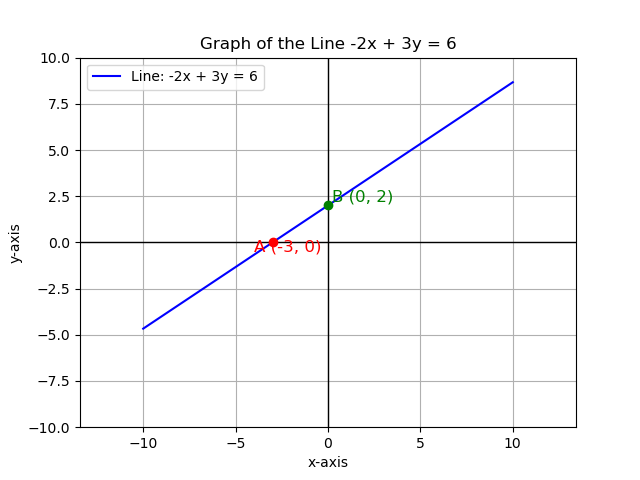
\includegraphics[width=\columnwidth, height=0.8\textheight, keepaspectratio]{Figure_6.png}     
\end{frame}
\end{document}